%%%%%%%%%%%%%%%%%%%%%%%%%%%%%%%%%%%%%%%%%%%%%%%%%%%%%%%%%%%%%%%%%
% MUW Presentation
% LaTeX Template
% Version 1.0 (27/12/2016)
%
% License:
% CC BY-NC-SA 4.0 (http://creativecommons.org/licenses/by-nc-sa/3.0/)
%
% Created by:
% Nicolas Ballarini, CeMSIIS, Medical University of Vienna
% nicoballarini@gmail.com
% http://statistics.msi.meduniwien.ac.at/
%
% Customized for UAH by:
% David F. Barrero, Departamento de Automática, UAH
%%%%%%%%%%%%%%%%%%%%%%%%%%%%%%%%%%%%%%%%%%%%%%%%%%%%%%%%%%%%%%%%%

\documentclass[10pt,compress]{beamer} % Change 10pt to make fonts of a different size
\mode<presentation>

\usepackage[spanish]{babel}
\usepackage{fontspec}
\usepackage{tikz}
\usepackage{etoolbox}
\usepackage{xcolor}
\usepackage{xstring}
\usepackage{listings}

% Introduced by David
\usepackage{eurosym}

\usetheme{UAH}
\usecolortheme{UAH}
\setbeamertemplate{navigation symbols}{} 
\setbeamertemplate{caption}[numbered]

%%%%%%%%%%%%%%%%%%%%%%%%%%%%%%%%%%%%%%%%%%%%%%%%%%%%%%%%%%%%%%%%%
%% Presentation Info
\title[Videogame engine architecture]{Videogame engine architecture}
\author{}
\institute{\asignatura}
\date{}
%%%%%%%%%%%%%%%%%%%%%%%%%%%%%%%%%%%%%%%%%%%%%%%%%%%%%%%%%%%%%%%%%


%%%%%%%%%%%%%%%%%%%%%%%%%%%%%%%%%%%%%%%%%%%%%%%%%%%%%%%%%%%%%%%%%
%% Descomentar para habilitar barra de navegación superior
\setNavigation
%%%%%%%%%%%%%%%%%%%%%%%%%%%%%%%%%%%%%%%%%%%%%%%%%%%%%%%%%%%%%%%%%

%%%%%%%%%%%%%%%%%%%%%%%%%%%%%%%%%%%%%%%%%%%%%%%%%%%%%%%%%%%%%%%%%
%% Configuración de logotipos en portada
%% Opacidad de los logotipos
\newcommand{\opacidad}{1}
%% Descomentar para habilitar logotipo en pié de página de portada
\renewcommand{\logoUno}{Images/isg.png}
%% Descomentar para habilitar logotipo en pié de página de portada
%\renewcommand{\logoDos}{Images/CCLogo.png}
%% Descomentar para habilitar logotipo en pié de página de portada
%\renewcommand{\logoTres}{Images/ALogo.png}
%% Descomentar para habilitar logotipo en pié de página de portada
%\renewcommand{\logoCuatro}{Images/ELogo.png}
%%%%%%%%%%%%%%%%%%%%%%%%%%%%%%%%%%%%%%%%%%%%%%%%%%%%%%%%%%%%%%%%%

%%%%%%%%%%%%%%%%%%%%%%%%%%%%%%%%%%%%%%%%%%%%%%%%%%%%%%%%%%%%%%%%%
%% FOOTLINE
%% Comment/Uncomment the following blocks to modify the footline
%% content in the body slides. 


%% Option A: Title and institute
\footlineA
%% Option B: Author and institute
%\footlineB
%% Option C: Title, Author and institute
%\footlineC
%%%%%%%%%%%%%%%%%%%%%%%%%%%%%%%%%%%%%%%%%%%%%%%%%%%%%%%%%%%%%%%%%

\begin{document}

%%%%%%%%%%%%%%%%%%%%%%%%%%%%%%%%%%%%%%%%%%%%%%%%%%%%%%%%%%%%%%%%%
% Use this block for a blue title slide with modified footline
{\titlepageBlue
    \begin{frame}
        \titlepage
    \end{frame}
}

\begin{frame}[plain]{}
   \begin{block}{Objectives}
   \begin{itemize}
        \item Introduce the main videogame subsystems
        \item Deep understanding of the main loop
        \item Describe different main loop implementation methods
	\end{itemize}
	\end{block}

   \begin{block}{Bibliography}
      \begin{enumerate}
          \item  \textit{Desarrollo de Videojuegos, Arquitectura del Motor de Videojuegos}. Capitulo 1, sección 2. UCLM.
      \end{enumerate} 
   \end{block}
\end{frame}

{
\disableNavigation{white}
\begin{frame}[shrink]{Table of Contents}
 \frametitle{Table of Contents}
 \tableofcontents
  % You might wish to add the option [pausesections]
\end{frame}
}

\section{Videogame engine architecture}
\subsection{Overview}
\begin{frame}{Videogame engine architecture}{Overview}
	Videogame engines aims to be independent of the game genre
	\begin{itemize}
		\item Increased design complexity
	\end{itemize}

	Videogame engines are complex systems $\Rightarrow$ Layered structure
	\begin{itemize}
		\item Layered architectures are common in complex systems
		\item Handle complexity
		\item Upper layers use services from the bottom layers
		\item Lower layers never access upper layers
		\item Adding layers is simple (well, more or less)
		\item One layer can be modified independently of the others
	\end{itemize}

	Other examples of layered structures: TCP/IP, OSI, operating systems
\end{frame}

\subsection{Conceptual overview of a videogame engine}
\begin{frame}[plain]{Videogame engine architecture}{Conceptual overview of a videogame engine}
	\begin{center}
		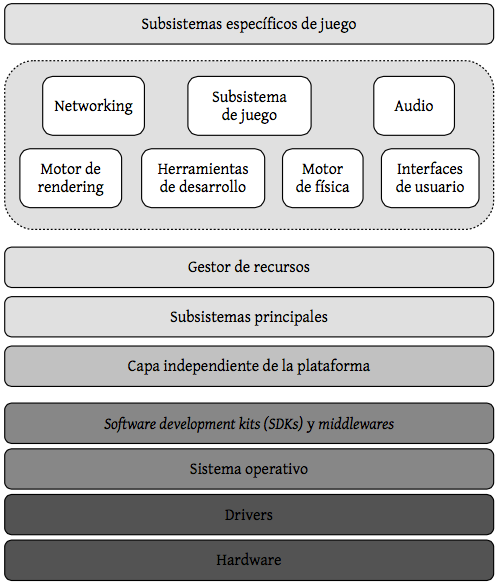
\includegraphics[width=0.6\linewidth]{figs/layers}
	\end{center}
\end{frame}

\subsection{Videogame engine layers}
\begin{frame}[plain]{Videogame engine architecture}{Videogame engine layers (I)}
	\begin{enumerate}
	\item \textbf{Hardware:} General purpose (PCs) or specific (consoles)
		\begin{itemize}
		\item The boundaries tend to vanish ...
		\end{itemize}
	\item \textbf{Drivers:} Interface between processes and hardware
	\item \textbf{Operating system:} Manages access to hardware
	\item \textbf{SDK and middlware:} General features not integrated in the OS
		\begin{itemize}
		\item OpenGL, Direct3D, authentication, etc
		\end{itemize}
	\item \textbf{Platform independent layer:} Isolates upper layer from the platform
		\begin{itemize}
		\item Encourages multiplatform games
		\end{itemize}
	\item \textbf{Main subsystems:} Some basic libraries not dependent on the videogame
		\begin{itemize}
		\item Mathematical library
		\item Datastructures and algorithms
		\item Memory management
		\item Debugging and logging
		\end{itemize}
	\end{enumerate}
\end{frame}

\begin{frame}[plain]{Videogame engine architecture}{Videogame engine layers (II)}
	\begin{enumerate}
	\setcounter{enumi}{6}
	\item \textbf{Resource manager:} Unified interface to access videogame resources
		\begin{itemize}
		\item Many game engines do not implement this
		\end{itemize}
	\item \textbf{Main subsystems:} General purpose (PCs) or specific (consoles)
		\begin{itemize}
		\item The boundaries tend to vanish ...
		\end{itemize}
	\item \textbf{Resource manager:} Manages access to hardware
	\item \textbf{SDK and middlware:} General purpose libraries
		\begin{itemize}
		\item OpenGL, Direct3D, etc
		\end{itemize}
	\item \textbf{Platform independent layer:} Isolates upper layer from the platform
		\begin{itemize}
		\item Encourages multiplatform games
		\end{itemize}
	\end{enumerate}
\end{frame}

\begin{frame}[plain]{Videogame engine architecture}{Videogame engine layers (III)}
    \begin{columns}
 	   \column{.65\textwidth}
	\begin{enumerate}
	\setcounter{enumi}{11}
	\item \textbf{Game specific subsystems:} 
		\begin{itemize}
		\item Physics engine
			\begin{itemize}
			\item Solid state physics \href{https://www.youtube.com/watch?v=PfezSJB21vk}{(Video 1)} \href{https://www.youtube.com/watch?v=q0xCYm6B9yE}{(Video 2)} \href{https://www.youtube.com/watch?v=Nj9TGIrgGVI}{(Video fails)}\\
			Havoc, PhysX, Bullet, ODE\\
			\item Particle physics \href{https://www.youtube.com/watch?v=x8Fo2slT2WA}{(Video 1)} \href{https://www.youtube.com/watch?v=Jl54WZtm0QE}{(Video 2)}
			\end{itemize}
		\item Collisions engine (usually integrated in physics)
			\begin{enumerate}[i]
			\item Collision detection
			\item Collision determination
			\item Collision handling
			\end{enumerate}
		\item User interface (UI)
		\item Networking
		\item Audio
		\item Rendering engine
		\end{itemize}
	\end{enumerate}
 	   \column{.3\textwidth}
			\centering
\includegraphics[width=0.9\linewidth]{figs/havok}\\\smallskip
			\centering
\includegraphics[width=0.9\linewidth]{figs/physx.png}\\\smallskip
			\centering
\includegraphics[width=0.9\linewidth]{figs/bullet}
 	   \column{.05\textwidth}
	\end{columns}
\end{frame}



\section{Videogame models}
\subsection{Render loop}
\begin{frame}{Videogame models}{Render loop (I)}
    \begin{columns}
 	   \column{.5\textwidth}
		\begin{itemize}
		\item Part of the rendering engine subsystem
	   	\item The render loop handles visualization and rendering
	   	\item Objectives in 2D games
		\begin{itemize}
			\item Minimize pixels to draw: Draw only those pixels that have changed
			\item Maximize fps
		\end{itemize}
		\end{itemize}
 	   \column{.5\textwidth}
	\centering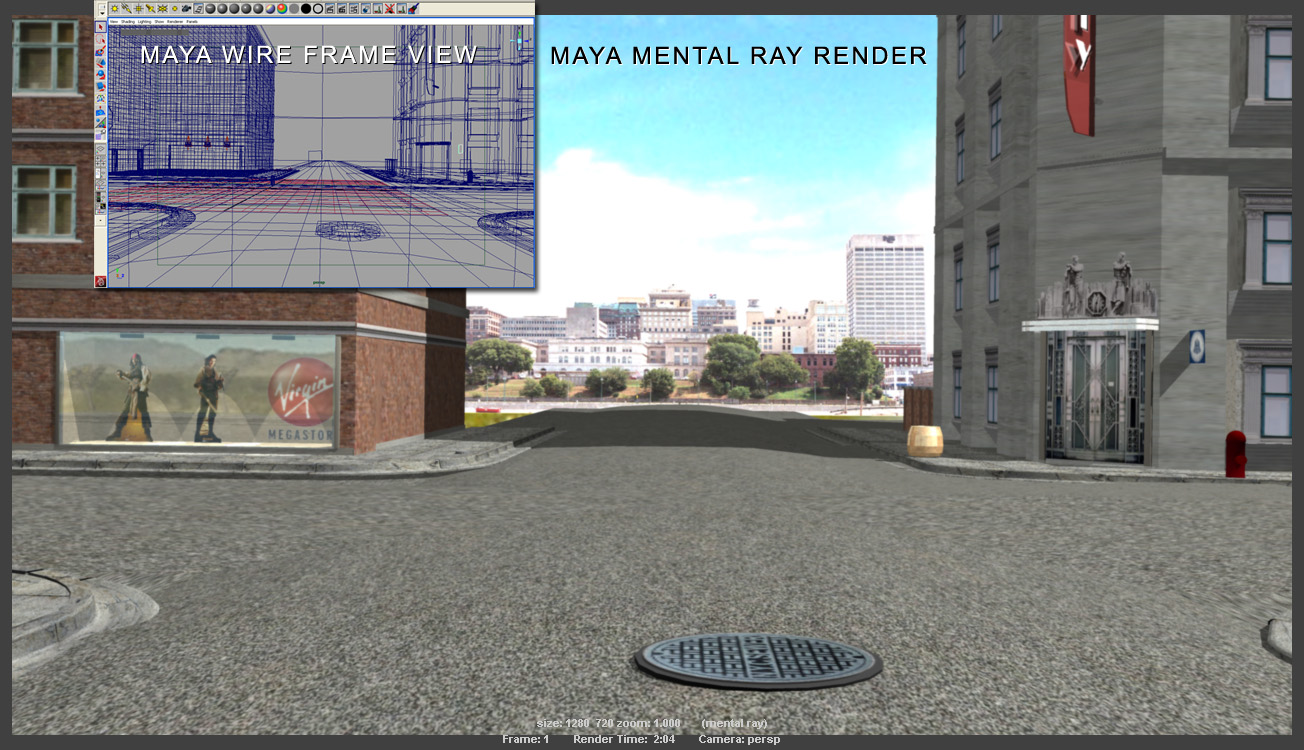
\includegraphics[width=0.8\linewidth]{figs/rendering}\\
	Render example
 	\end{columns}
	\begin{itemize}
	\item Objectives in 3D games
		\begin{itemize}
			\item Camera uses to change everytime: The same technique cannot be used
			\item Minimize the number of primites to draw in each iteration of the render loop
		\end{itemize}
	\end{itemize}
\end{frame}

\begin{frame}{Videogame models}{Render loop (II)}
	    \vspace{-0.2cm}
    \begin{block}{Render loop}
	    \vspace{-0.2cm}
	    \lstinputlisting[language=java, basicstyle=\ttfamily\scriptsize]{code/renderloop.java}
		\vspace{-0.2cm}
	\end{block}
	Info: \url{http://wiki.wxwidgets.org/Making\_a\_render\_loop}
\end{frame}


\subsection{Game loop}
\begin{frame}{Videogame models}{Game loop (I)}
	   	The main element in a videogame is the \alert{game loop}
		\begin{itemize}
			\item It is the main control structure in the game
			\item It controls its execution
			\item It handlers the transitions among states
			\item The game loop independizes the game execution from the hardware
		\end{itemize}
		Classical programs only reacts with user actions
		\begin{itemize}
			\item Videogames are always performing an action
			\item Game loop implements this easely
			\item The game engine contains the game loop
		\end{itemize}
\end{frame}

\begin{frame}{Videogame models}{Game loop (II)}
		\begin{itemize}
		   	\item There are many subsystems in a videogame
			\begin{itemize}
				\item Rendering engine
				\item Physics and collision detection
				\item AI subsystem
				\item Game subsystem
			\end{itemize}
			\item Most of these subsystems require periodic updates
			\item The most critical one is the animation system
			\begin{itemize}
				\item Frequency: 30 or 60 Hz
				\item Syncronized with the rendering subsystem
				\item Objective: Provide a good fps rate to generate a realistic experience
			\end{itemize}
			\item Not all the components are so strict, for instance, AI
		\end{itemize}
\end{frame}

\begin{frame}{Videogame models}{Game loop (III)}
	\begin{itemize}
	   	\item There are several ways to implement the game loop
	   	\item The easiest one is to have several loops within the game loop
		\begin{itemize}
			\item Render loop
			\item AI loop
			\item Multimedia loop
			\item Iteration loop
		\end{itemize}
	\end{itemize}

    \begin{columns}
 	   \column{.4\textwidth}
    \begin{block}{Basic game loop}
	    \vspace{-0.2cm}
	    \lstinputlisting[language=java, basicstyle=\ttfamily\scriptsize]{code/gameloop1.java}
		\vspace{-0.2cm}
	\end{block}
   \column{.6\textwidth}
    \begin{block}{Game loop}
	    \vspace{-0.2cm}
	    \lstinputlisting[language=java, basicstyle=\ttfamily\scriptsize]{code/gameloop2.java}
		\vspace{-0.2cm}
	\end{block}
	\end{columns}
\end{frame}

\begin{frame}{Videogame models}{Game loop (IV)}
	    \vspace{-0.3cm}
    \begin{columns}
 	   \column{.7\textwidth}
    \begin{block}{}
	    \vspace{-0.2cm}
	    \lstinputlisting[language=c, basicstyle=\ttfamily\scriptsize]{code/pong.c}
		\vspace{-0.2cm}
	\end{block}
   \column{.3\textwidth}
   	Pong game loop example
	\centering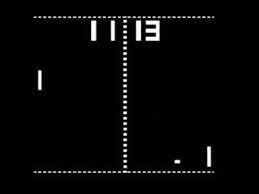
\includegraphics[width=\linewidth]{figs/pong.jpeg}
	\end{columns}
\end{frame}

\begin{frame}[plain]{Videogame models}{Game loop (V)}
	\centering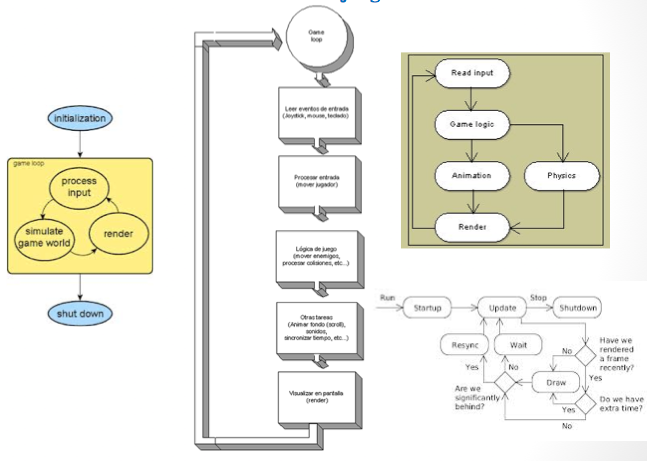
\includegraphics[width=\linewidth]{figs/gameloops}
\end{frame}

\begin{frame}{Videogame models}{Game loop (VI)}
	    The game loop depends on the platform
		\begin{itemize}
			\item DOS games and some consoles are designed to exploit computational resources
			\item PC games depend on limitations imposed by the OS
			\item Games use to be multithreaded to exploit multicore machines
		\end{itemize}

		\begin{block}{Exercise}
			\begin{enumerate}
			\item Open the Space Invaders source code available on \\
			\url{https://github.com/leerob/Space_Invaders/blob/master/spaceinvaders.py}
			\item Locate the game main loop
			\end{enumerate}
		\end{block}
\end{frame}

\section{Game architectures}
\subsection{Game architectures}

\begin{frame}{Game architectures}{Game architectures}
    Game loop can be implemented in different ways
	\begin{itemize}
		\item Architectures based on callbacks
		\item Architectures based on events
		\item Architectures based on state machines
	\end{itemize}
	Most of them implement one or more control loops
\end{frame}

\subsection{Callbacks}
\begin{frame}{Game architectures}{Callbacks (I)}
	\begin{itemize}
		\item \textbf{Callbacks}: Code that is executed to handle an event
		\begin{itemize}
			\item Function or object
			\item Callbacks are used to ``fill'' source code
		\end{itemize}
		\item Related term: \textbf{framework}
		\begin{itemize}
			\item Application partially completed that the developer has to complete
		\end{itemize}
	\end{itemize}
\end{frame}

\begin{frame}{Videogame models}{Callbacks (II)}
	\vspace{-0.3cm}
    \begin{columns}
 	   	\column{.9\textwidth}
    		\begin{block}{}
	    	\vspace{-0.2cm}
	    	\lstinputlisting[language=c, basicstyle=\ttfamily\scriptsize]{code/callback.c}
			\vspace{-0.2cm}
			\end{block}
	\end{columns}
\end{frame}

\subsection{Events}
\begin{frame}{Game architectures}{Events}
	\begin{itemize}
		\item An event represents a change in the game state
		\item Two types
		\begin{itemize}
			\item \textbf{External}: Generated by the interactions\\Example, The player press a key or moves the joystick
			\item \textbf{Internal}: Generated by the game logic\\Example, NPC respawn
		\end{itemize}
		\item Most game engines include an event subsystem
		\begin{itemize}
			\item Closely related to the \textit{Observer} pattern
		\end{itemize}

	\end{itemize}
\end{frame}

\subsection{State machine}
\begin{frame}{Game architectures}{State machine}
	\vspace{-0.3cm}
	A game goes through a number of \alert{states}
		\begin{itemize}
			\item Introduction
			\item Main menu
			\item Game
			\item Game over
		\end{itemize}
	\textbf{State machine}: A set of states and transitions
	\vspace{0.3cm}
	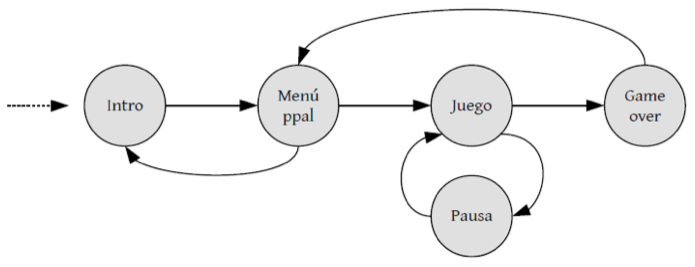
\includegraphics[width=0.7\linewidth]{figs/states}\\
	\vspace{-0.2cm}
	Warning: State machines play a mayor role in game AI
\end{frame}



\end{document}
